\section{Results}
Lorem Ipsum

\begin{figure}
	\begin{center}
		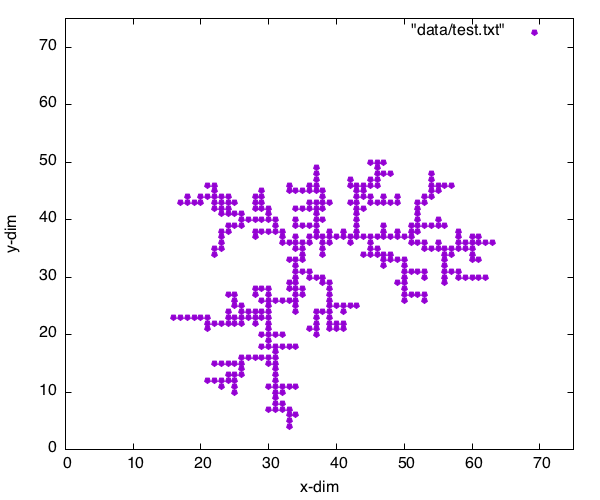
\includegraphics[width = 0.8\textwidth]{fig/on_lattice_400_p_75_g.png}
		\label{fig:2d-DLA_400}
		\caption{\textcolor{red}{??? I'm sure there could be some improvements to this.} On-lattice DLA simulation of 400 particles on a 75 by 75 grid.  This particular cluster has a fractal dimension of $d_f = 1.70999$.}
	\end{center}
\end{figure}

\begin{figure}
	\begin{center}
		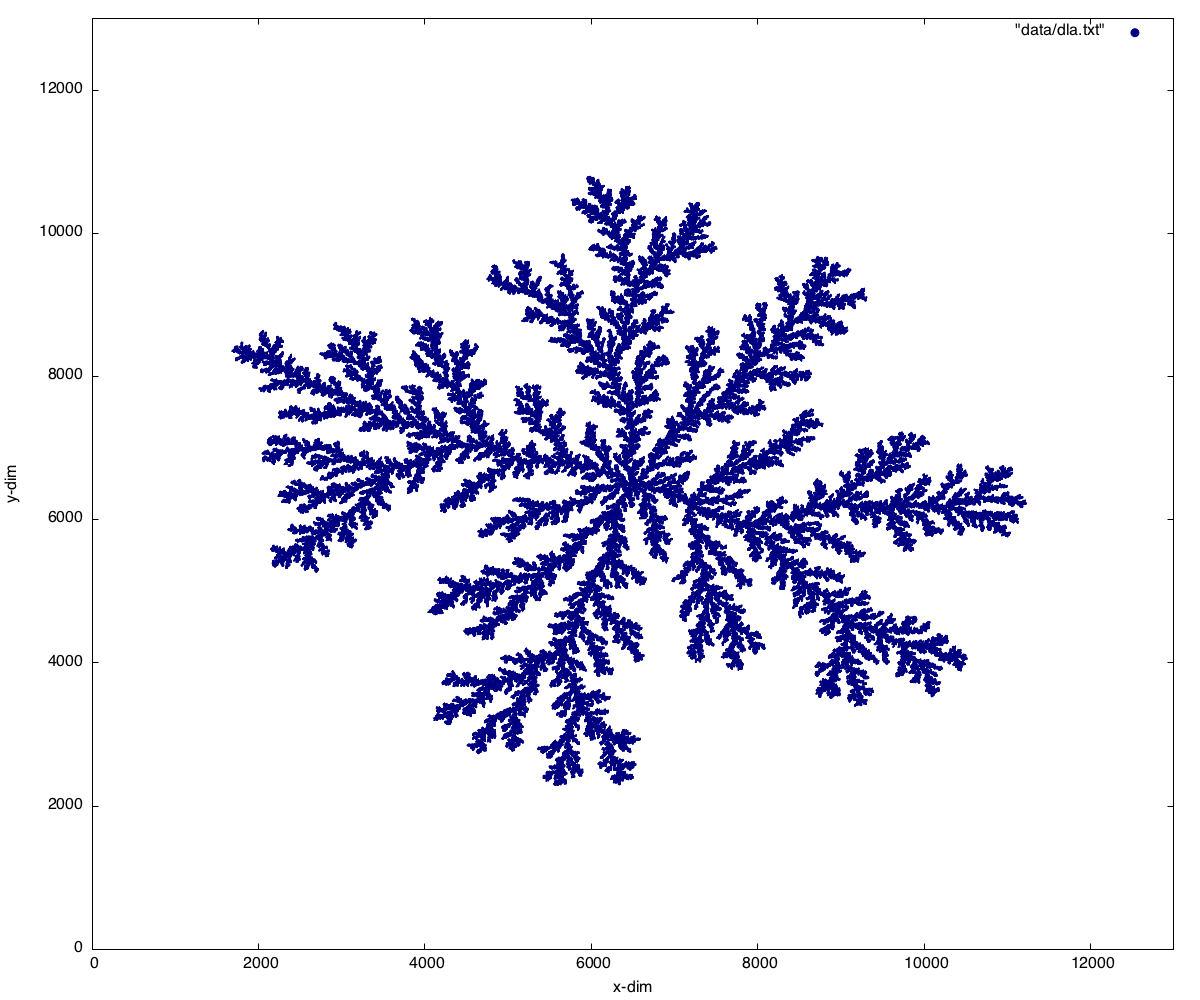
\includegraphics[width = 0.8\textwidth]{fig/1_(1_71348).png}
		\label{fig:2d-DLA_1mill}
		\caption{\textcolor{red}{??? Replace with a borderless version, so that one doesn't have to have x-ticks and x-labels etc...} Off-lattice DLA simulation of $10^6$ particles. This particular cluster has a fractal dimension of $d_f = 1.71348$.}
	\end{center}
\end{figure}

\begin{figure}
	\begin{center}
		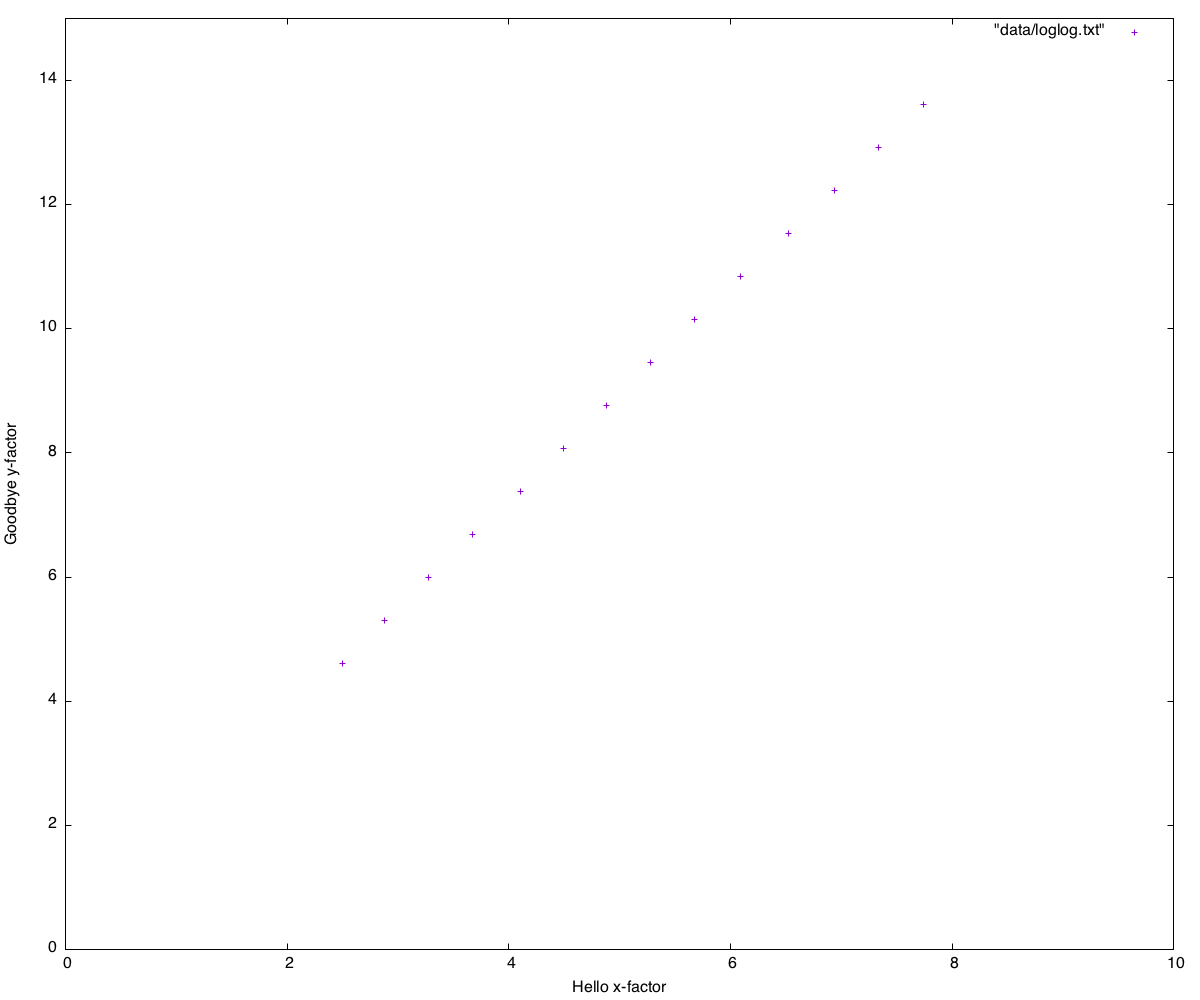
\includegraphics[width = 0.8\textwidth]{fig/loglog.png}
		\label{fig:loglog2d-DLA_1mill}
		\caption{The log-log plot of $N$ and $R_g$. From this, the fractal dimension was calculated using linear regression.  \textcolor{red}{??? replace with a plot including the slope/linear approximation.}}
	\end{center}
\end{figure}
